
\section{Auswertung}
\label{sec:Auswertung}
In diesem Abschnitt werden die aufgenommenen Messdaten in Grafiken sowie Tabellen dargestellt und ausgewertet. Grafiken sowie dazugehörige Rechnungen sind mit Python \cite{python} erstellt bzw. berechnet worden.
\subsection{Bestimmung des Untergrundes}
\label{sec:unter}
Um den Untergrund zu bestimmen wird die Gaußglocke aus den aufgenommenen Daten ausgeschlossen und es wird eine Ausgleichsrechnung der Form
\begin{equation*}
  I(T)=a\cdot T+b
\end{equation*}
durchgeführt. Ein exponentieller Fit ließ sich leider nicht durchführen. In Abbildung (\ref{fig:1}) sind die Daten für die erste Heizrate von $\SI{1.99(32)}{\kelvin\per\minute}$ und in Abbildung (\ref{fig:2}) für die zweite Heizrate von $\SI{1.48(31)}{\kelvin\per\minute}$ dargestellt. Die Heizraten sind aus dem Mittelwert der mittleren Änderungsraten zwischen zwei Messdaten bestimmt.
\begin{figure}[h!]
  \centering
  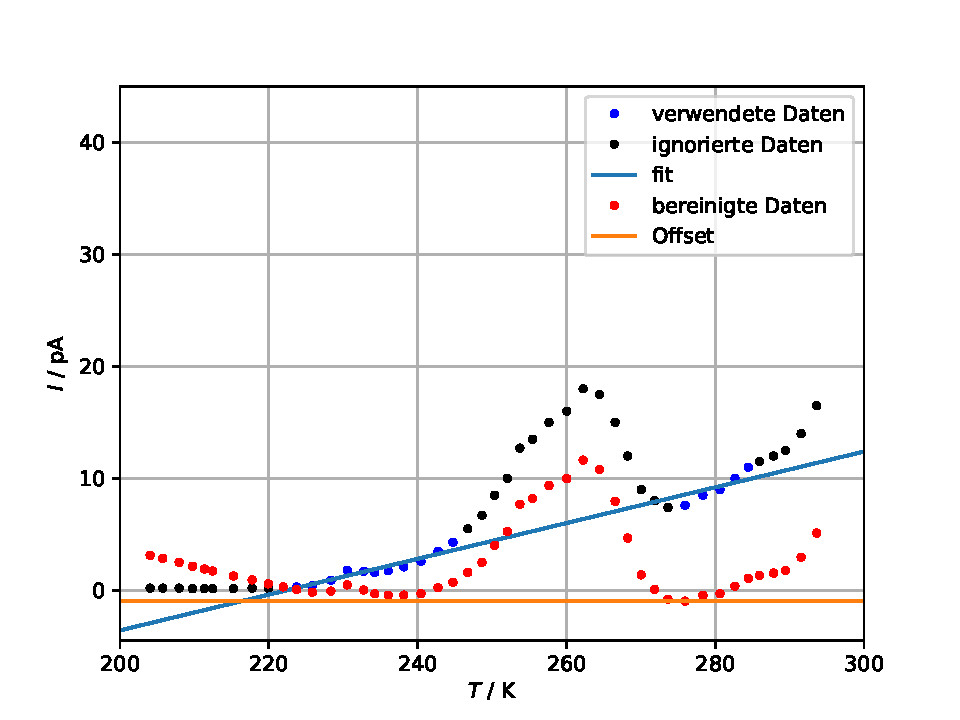
\includegraphics[scale=0.8]{fig/plot1.pdf}
  \caption{Depolarisationsstrom aufgetragen gegen die Temperatur für eine Heizrate von $\SI{1.99(32)}{\kelvin\per\minute}$}
  \label{fig:1}
\end{figure}
\begin{figure}[h!]
  \centering
  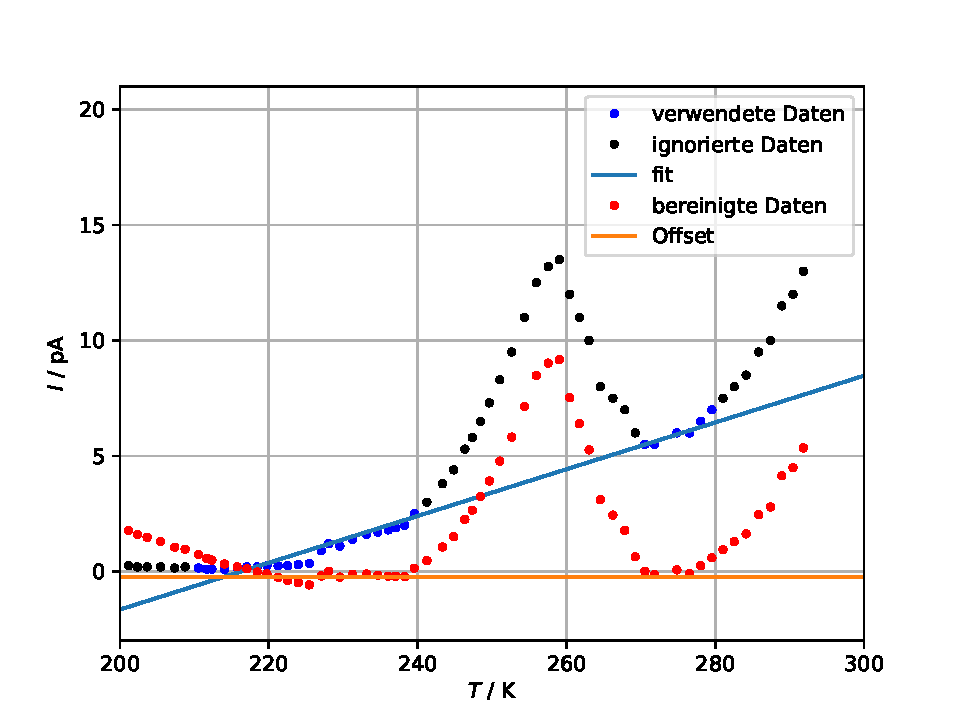
\includegraphics[scale=0.8]{fig/plot2.pdf}
  \caption{Depolarisationsstrom aufgetragen gegen die Temperatur für eine Heizrate von $\SI{1.48(31)}{\kelvin\per\minute}$}
  \label{fig:2}
\end{figure}
\FloatBarrier
Die Parameter ergeben sich für die erste Heizrate zu:
\begin{align*}
    a_\mathrm{1} &= \SI{0.159(5)e-12}{\ampere\per\kelvin} \\
    b_\mathrm{1} &= \SI{-35(1)e-12}{\ampere}.
\end{align*}
und für die zweite Heizrate zu:
\begin{align*}
    a_\mathrm{2} &= \SI{0.101(2)e-12}{\ampere\per\kelvin} \\
    b_\mathrm{2} &= \SI{-21.9(7)e-12}{\ampere}.
\end{align*}
\subsection{Berechnung der Aktivierungsenergie}
In diesem Abschnitt wird die Aktivierungsenergie mithilfe der zwei verschiedenen Ansätzen aus dem Abschnitt (\ref{sec:akti}) bestimmt.
\subsubsection{Polarisationsansatz}
In den Abbildungen (\ref{fig:3}) und (\ref{fig:4}) sind die verwendeten Daten für die Berechnung der Aktivierungsenergie $W$ für die zwei verschiedenen Heizraten dargestellt.
\begin{figure}[h!]
  \centering
  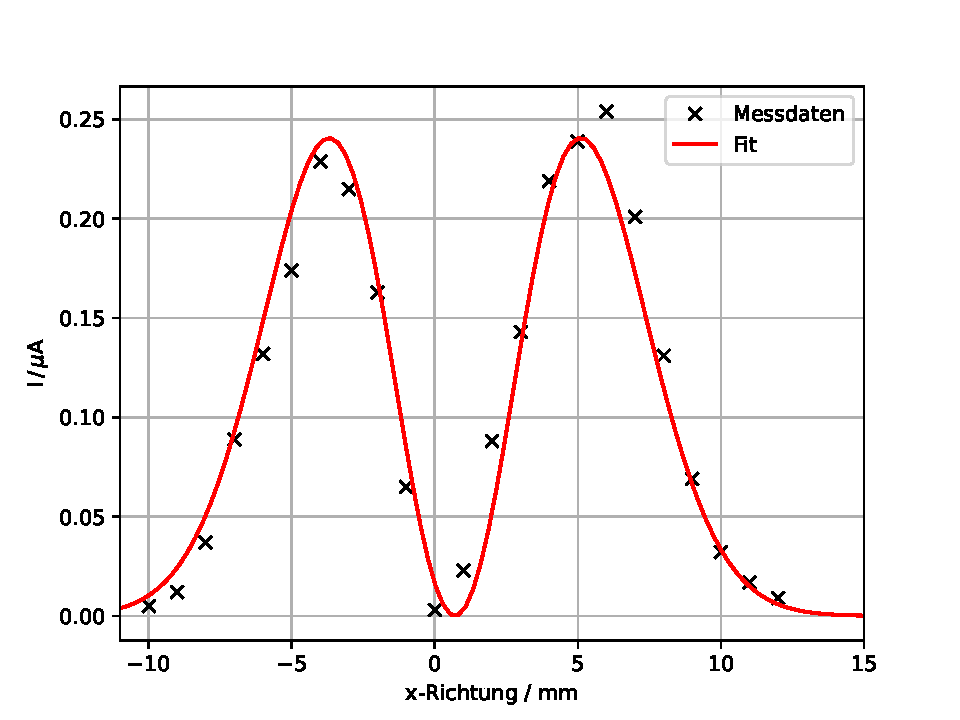
\includegraphics[scale=0.8]{fig/plot3.pdf}
  \caption{Halblogarithmische Darstellung des Polarisationsstroms gegen den Kehrwert der Temperatur für eine Heizrate von $\SI{1.99(32)}{\kelvin\per\minute}$}
  \label{fig:3}
\end{figure}
\begin{figure}[h!]
  \centering
  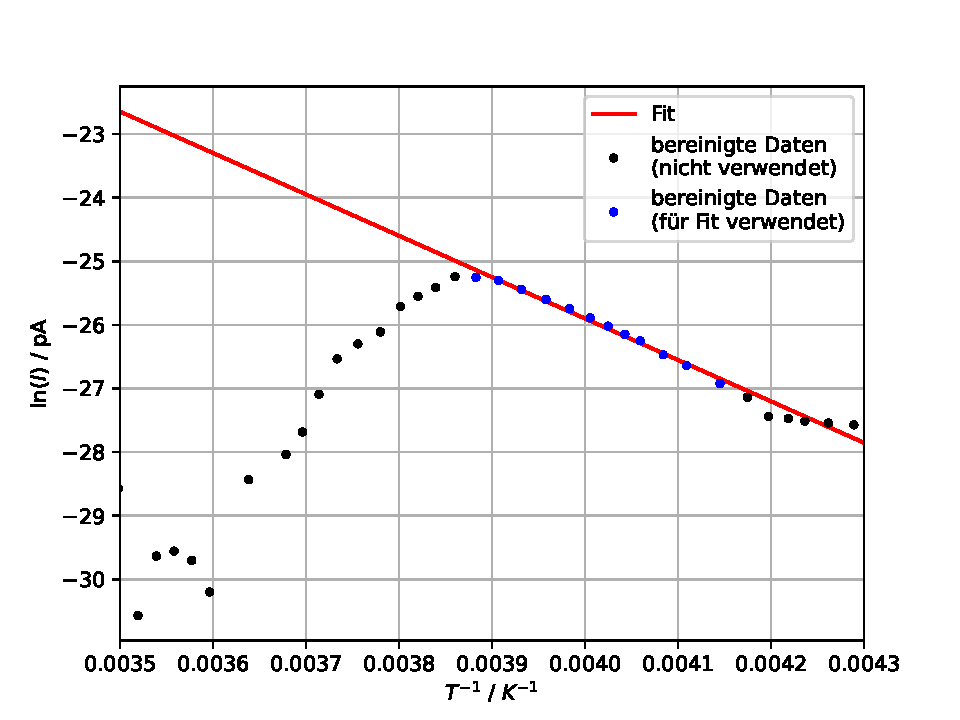
\includegraphics[scale=0.8]{fig/plot4.pdf}
  \caption{Halblogarithmische Darstellung des Polarisationsstroms gegen den Kehrwert der Temperatur für eine Heizrate von $\SI{1.48(31)}{\kelvin\per\minute}$}
  \label{fig:4}
\end{figure}
\FloatBarrier
Es wird wie aus Abschnitt (\ref{sec:polaris}) folgt eine Ausgleichsrechnung der Form
\begin{equation}
    \label{eqn:lin}
    \ln\left(\dfrac{I(T)}{\SI{1e-11}{\ampere}}\right) = -\dfrac{W}{k_\mathrm{B} T} + c,
\end{equation}
durchgeführt.
Daraus ergeben sich die Parameter zu:
\begin{align*}
    W_\mathrm{1} &= \SI{0.88(5)}{\electronvolt} \\
    W_\mathrm{2} &= \SI{0.83(5)}{\electronvolt} \\
    c_\mathrm{1} &= \num{14(2)} \\
    c_\mathrm{2} &= \num{12(2)}
\end{align*}
\subsubsection{Berechung über die Stromdichte}
In diesem Abschnitt wird die Methode aus Abschnitt (\ref{sec:strom1}) verwendet um die Aktivierungsenergie zu bestimmen. Die Messdaten sind in Abbildung (\ref{fig:5}) für die erste Heizrate und in Abbildung (\ref{fig:6}) dargestellt.
\begin{figure}[h!]
  \centering
  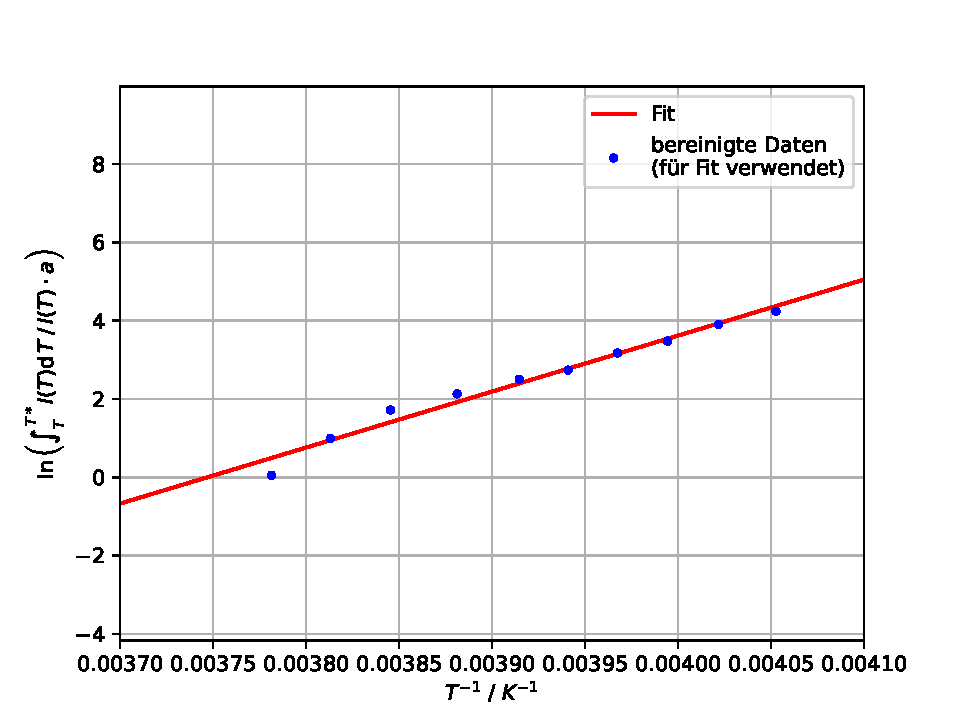
\includegraphics[scale=0.8]{fig/plot5.pdf}
  \caption{Integrierter Polarisationsstrom gegen den Kehrwert der Temperatur für eine Heizrate von $\SI{1.99(32)}{\kelvin\per\minute}$}
  \label{fig:5}
\end{figure}
\begin{figure}[h!]
  \centering
  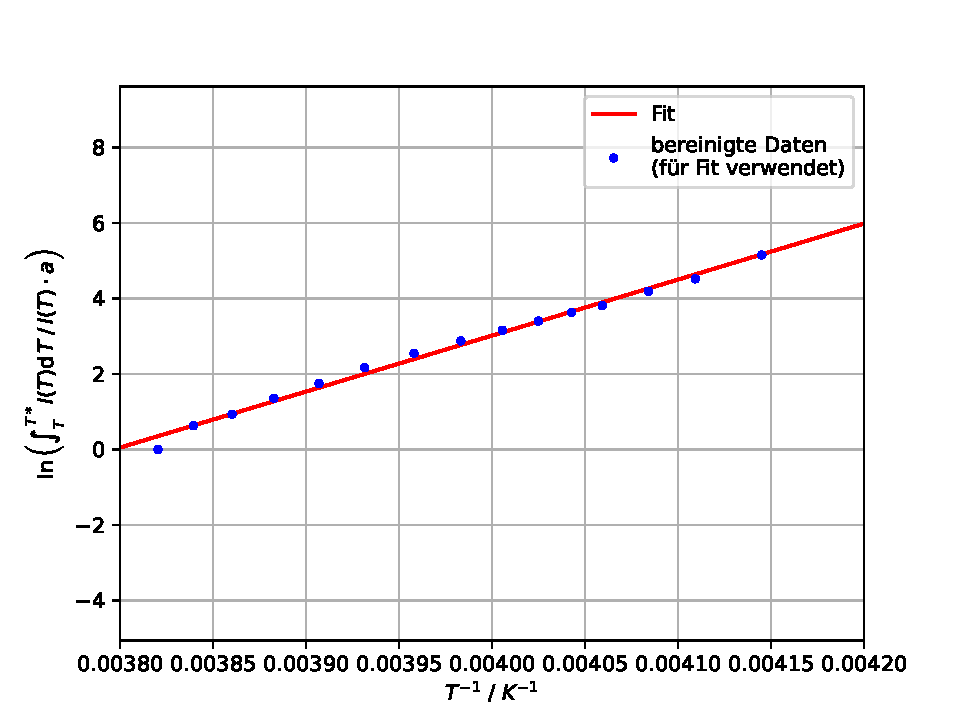
\includegraphics[scale=0.8]{fig/plot6.pdf}
  \caption{Integrierter Polarisationsstrom gegen den Kehrwert der Temperatur für eine Heizrate von $\SI{1.48(31)}{\kelvin\per\minute}$}
  \label{fig:6}
\end{figure}
\FloatBarrier
Für die Berechnung wird der Ausdruck
\begin{align*}
      \int_T^{T^*} I(T') \symup{d}\,T'
\end{align*}
numerisch integriert. Es soll gelten $I(T^*)\approx\SI{0}{\ampere}$. Daraus folgt für die erste Heizrate $T^*=\SI{275.95}{\kelvin}$ und für die zweite Heizrate $T^*=\SI{271.85}{\kelvin}$.
Der Ausdruck
\begin{align*}
   \ln\left(\frac{\int_T^{T^*} I(T') \symup{d}\,T'}{a_i \cdot I(T)}\right)
\end{align*}
wird gegen den Kehrwert der Temperatur aufgetragen und es wird wieder eine lineare Ausgleichsrechnung der Form
\begin{equation*}
  \ln\left(\frac{\int_T^{T^*} I(T') \symup{d}\,T'}{a_i \cdot I(T)}\right)=\dfrac{W}{k_\mathrm{b}T}+d
\end{equation*}
durchgeführt. Damit ergeben sich folgende Werte:
\begin{align*}
    W_\mathrm{1} &= \SI{1.23(7)}{\electronvolt} \\
    W_\mathrm{2} &= \SI{1.27(3)}{\electronvolt} \\
    d_\mathrm{1} &= \num{-54(3)} \\
    d_\mathrm{2} &= \num{-56(1)}
\end{align*}
\subsection{Relaxationszeit}
\label{sec:88}
Die charakteristische Relaxationszeit lässt sich aus dem Maximum bestimmen mit:
\begin{equation}
  \tau_\mathrm{0}=\dfrac{\symup{k_B}T_\mathrm{max}^2}{W \cdot b} \exp\left(-\dfrac{W}{\symup{k_B}T_\mathrm{max}} \right)
\end{equation}
Die Relaxationszeiten ergeben sich demnach für die erste Heizrate zu
\begin{align*}
  \tau_\mathrm{0}(\mathrm{Polarisation})&= \SI{4(9)e-17}{\second} \\
  \tau_\mathrm{0}(\mathrm{Stromdichte})&= \SI{1(2)e-23}{\second}
\end{align*}
und für die zweite Heizrate zu
\begin{align*}
  \tau_\mathrm{0}(\mathrm{Polarisation})&= \SI{4(9)e-16}{\second} \\
  \tau_\mathrm{0}(\mathrm{Stromdichte})&= \SI{4(6)e-25}{\second}
\end{align*}
